\chapter{出生、生长与死亡}\label{ch:g2:born-grow-die}

春天，门边的樱桃树开满了花；
树下，一只母猫正在喂养刚出生的小猫；爷爷
拿出一张他和你同龄时的照片——瘦小，缺了门牙，
已经很爱吃樱桃。每一种\omterm{def:g1:living-or-not:living}{生物}都走着同样的
道路：它开始，它生长，有一天它会结束。这条路被称为
\omterm{def:g2:born-grow-die:cycle}{生命周期}。

\section{生命的各个阶段}

\begin{definition}[生命周期]\label{def:g2:born-grow-die:cycle}
\omterm{def:g1:living-or-not:living}{生物}的\emph{生命周期}\index{生命周期}，是指它一生经历的
一系列\emph{阶段}\index{阶段}：
\begin{enumerate}
  \item 它\emph{出生}\index{出生}——开始；
  \item 它是\emph{幼体}\index{幼体}——正在生长，
        变化很快；
  \item 它是\emph{成体}\index{成体}——已经完全长大；成体
        能够生出自己的幼体；
  \item 它进入\emph{老年}\index{老年期}，最终
        \emph{死亡}\index{死亡}。
\end{enumerate}
\end{definition}

\begin{example}[三种生命，同一条道路]\label{ex:g2:born-grow-die:three}
一只小猫出生、玩耍，长成一只猫，
她自己也可能生下小猫，然后变老。一颗樱桃种子发芽，幼树
逐年长高，成年树开花、结樱桃，
经过几十年后死亡。而你：婴儿、儿童，然后
有一天成为大人。小猫、樱桃树、儿童——同样的四个
\omterm{def:g2:born-grow-die:cycle}{阶段}。
\end{example}

\begin{omfigure}
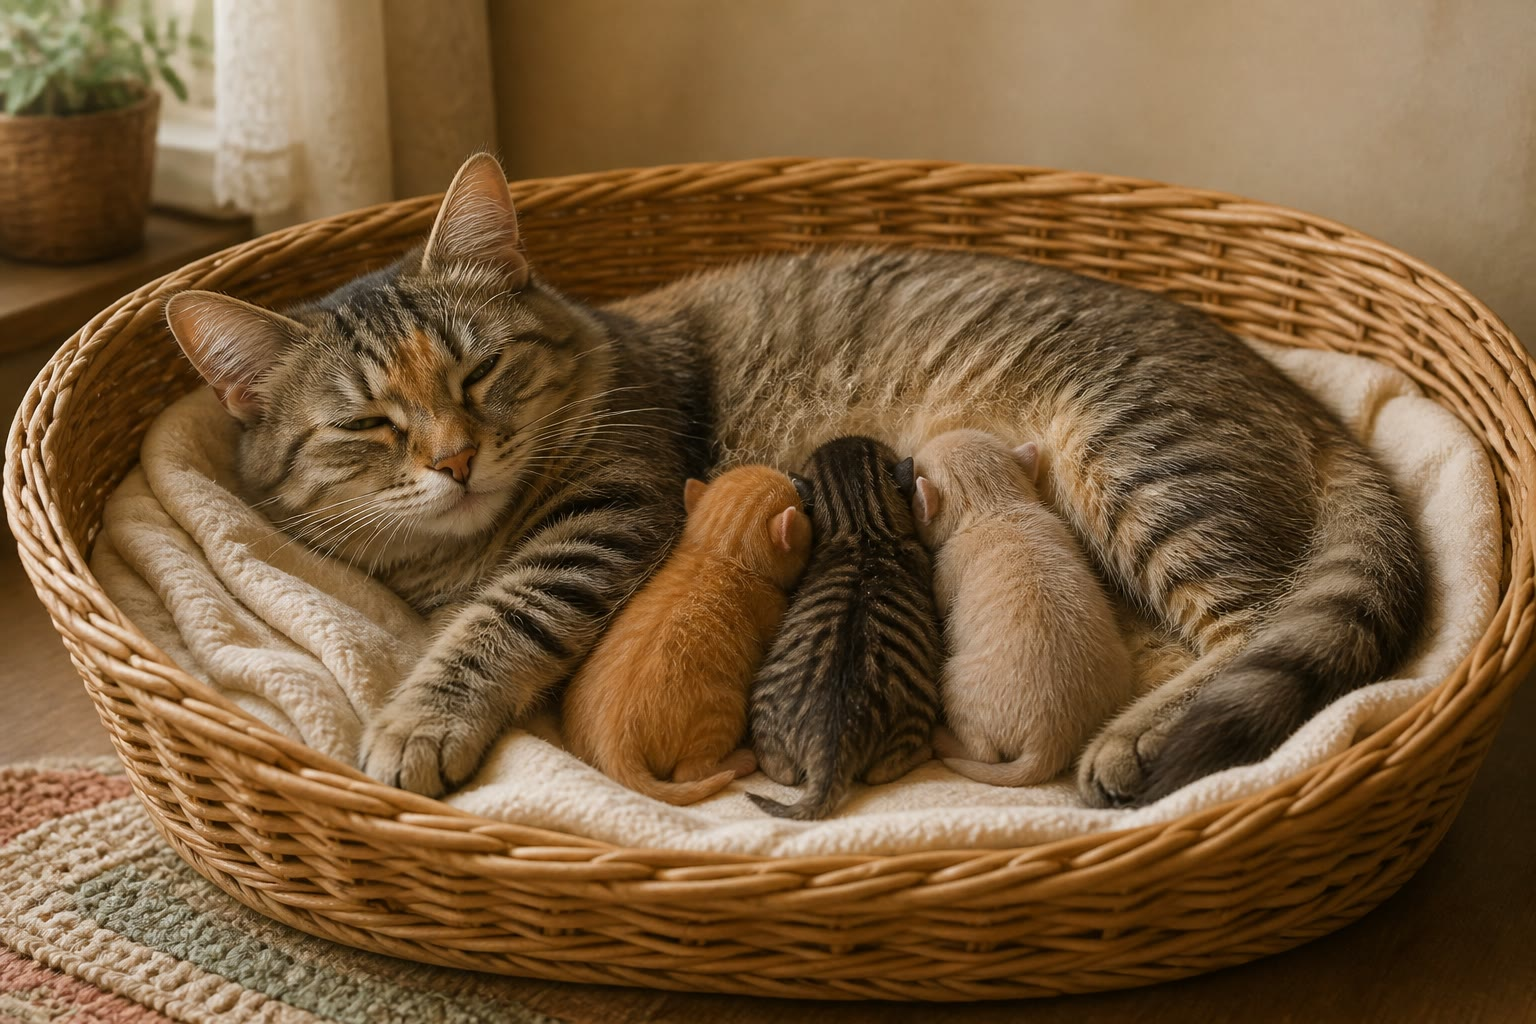
\includegraphics[width=0.62\linewidth]{images/book1/ai/g2-cycle-kittens.jpg}

{\small 三个\omterm{def:g2:born-grow-die:cycle}{生命周期}同时开始：刚出生的
小猫正在吃母猫的乳汁。}
\end{omfigure}

\begin{omfigure}
\begin{tikzpicture}[scale=0.92]
  \foreach \x/\txt in {0/{出生},3.1/{幼年},6.2/{成年},9.3/{老年}} {
    \draw[thick, omDef, fill=omDef!7, rounded corners=5pt]
      (\x,0) rectangle ({\x+2.4},1.2);
    \node[font=\small\bfseries, text height=1.6ex, text depth=0.4ex]
      at ({\x+1.2},0.6) {\txt};
  }
  \draw[->, thick, omMeth] (2.4,0.6) -- (3.1,0.6);
  \draw[->, thick, omMeth] (5.5,0.6) -- (6.2,0.6);
  \draw[->, thick, omMeth] (8.6,0.6) -- (9.3,0.6);
  % new generation arrow
  \draw[->, thick, omProp] (7.4,1.2) .. controls (7.4,2.3) and (1.2,2.3)
    .. (1.2,1.25);
  \node[font=\small, omProp] at (4.3,2.35) {成体会产下幼体：新的循环开始};
\end{tikzpicture}

{\small 生命的各个\omterm{def:g2:born-grow-die:cycle}{阶段}——以及引向下一代的箭头，
让生命之路再次开始。}
\end{omfigure}

\begin{remark}[为什么叫作循环]\label{rem:g2:born-grow-die:wheel}
每一段生命都从出生走到死亡，就像一条有两个
端点的路。但在终点之前，\omterm{def:g2:born-grow-die:cycle}{成体}会产下幼体，这些幼体
又开始新的旅程。从许多代来看，生命像一个
车轮一样转动——这正是我们把生命称为\emph{循环}的原因。
\end{remark}

\section{生长与变化}

\begin{proposition}[长大不只是变大]\label{prop:g2:born-grow-die:change}
\omterm{def:g1:living-or-not:living}{生物}在生长的同时，幼体也会\emph{变化}：婴儿
会长出牙，掉了又长出更结实的新牙；小鸡的黄色
绒毛变成真正的\omterm{def:g1:animals-around-us:covering}{羽毛}；幼树柔软的绿色茎
变成坚硬的木材。生长不只是变大，\emph{而且}变得
不同。
\end{proposition}
\admitted

\begin{example}[照片检验]\label{ex:g2:born-grow-die:photo}
在爷爷的旧照片中，你可以追踪一个人
经历的每个\omterm{def:g2:born-grow-die:cycle}{阶段}：婴儿、小学生、青年、父亲、爷爷。
同一个人，身体在变化。照片就像一台台小小的时光机，
用来观察一个\omterm{def:g2:born-grow-die:cycle}{生命周期}。
\end{example}

\begin{method}[将生命阶段排序]\label{met:g2:born-grow-die:order}
给出一组打乱顺序的\omterm{def:g1:living-or-not:living}{生物}一生的图片：
\begin{enumerate}
  \item 找出出生的图片——卵、种子或刚出生的婴儿；
  \item 找出\omterm{def:g2:born-grow-die:cycle}{成体}——已完全长大，能够生出幼体；
  \item 把幼体放在中间，从小到大排列；
  \item 检查你的排列：每张图片是否都能引出下一张？
\end{enumerate}
\end{method}

\section{每个生命都会结束——但生命仍在延续}

\begin{proposition}[寿命]\label{prop:g2:born-grow-die:lifespan}
不同的\omterm{def:g1:living-or-not:living}{生物}存活的时间长短不同——这叫
\emph{寿命}\index{寿命}。蝴蝶可能只活几周；
猫和狗一般活十到二十年；人通常可以活过
八十岁；有些树可以活几百年。无论长短，每个
生命都有终点。
\end{proposition}
\admitted

\begin{example}[老苹果树]\label{ex:g2:born-grow-die:oldtree}
花园尽头那棵弯曲的老苹果树，每年结的苹果越来越少——它已进入\omterm{def:g2:born-grow-die:cycle}{老年期}。
但它的苹果里有种子，一粒种子种下去，就已经是一棵幼小的苹果树，
开始这段旅程。老树死去时，
苹果树并不会
消失：它的幼体会延续下去。
\end{example}

\begin{remark}[谈论死亡]\label{rem:g2:born-grow-die:death}
死亡是每个生命循环的一部分，为此感到难过也是可以的——
人们确实会这样，尤其是为宠物和我们
所爱的人难过。生物学带来一点安慰：\omterm{def:g2:born-grow-die:cycle}{成体}
在死去之前会产下幼体，所以生命本身会一轮又一轮地延续下去。
\end{remark}

\section{练习}

\begin{exercise}[$\star$]\label{exo:g2:born-grow-die:1}
按顺序说出\omterm{def:g2:born-grow-die:cycle}{生命周期}的四个\omterm{def:g2:born-grow-die:cycle}{阶段}。
\end{exercise}

\begin{exercise}[$\star$]\label{exo:g2:born-grow-die:2}
\omterm{def:g1:living-or-not:living}{生物}在\omterm{def:g2:born-grow-die:cycle}{生命周期}的哪个\omterm{def:g2:born-grow-die:cycle}{阶段}能够生下自己的幼体？
\end{exercise}

\begin{exercise}[$\star$]\label{exo:g2:born-grow-die:3}
请按从年长到年幼排列：一名小学生、一个婴儿、
一位祖母、一位母亲。
\end{exercise}

\begin{exercise}[$\star$]\label{exo:g2:born-grow-die:4}
请写出下面这棵樱桃树的\omterm{def:g2:born-grow-die:cycle}{生命周期}，
并逐\omterm{def:g2:born-grow-die:cycle}{阶段}说明，樱桃树见\cref{ex:g2:born-grow-die:three}。
\end{exercise}

\begin{exercise}[$\star$]\label{exo:g2:born-grow-die:5}
请从\cref{prop:g2:born-grow-die:change}中举出两个例子，
说明一个幼小的\omterm{def:g1:living-or-not:living}{生物}在生长时发生\emph{变化}，
而不只是变大。
\end{exercise}

\begin{exercise}[$\star$]\label{exo:g2:born-grow-die:6}
通常谁活得更长：蝴蝶、猫，还是橡树？
请将这三者按\omterm{prop:g2:born-grow-die:lifespan}{寿命}长短排序。
\end{exercise}

\begin{exercise}[$\star$]\label{exo:g2:born-grow-die:7}
为什么要用\emph{循环}一词，既然每个生命都像一条路，
从出生走到死亡？请结合图中的紫色箭头说明。
\end{exercise}

\begin{exercise}[$\star$]\label{exo:g2:born-grow-die:8}
动手试一试：请家人找来一位成年人不同年龄时的照片，
并按\omterm{def:g2:born-grow-die:cycle}{生命周期}的顺序排列，排列方法见
\cref{met:g2:born-grow-die:order}。照片展示了哪些\omterm{def:g2:born-grow-die:cycle}{阶段}？
还有哪个\omterm{def:g2:born-grow-die:cycle}{阶段}尚未到来？
\end{exercise}

\begin{exercise}[$\star\star$]\label{exo:g2:born-grow-die:9}
\cref{ex:g2:born-grow-die:oldtree}中的老苹果树总有一天会死去，
但花园里不必失去苹果树。请解释原因，
可以用\emph{世代}一词作答，也可以借助
图中的紫色箭头说明。
\end{exercise}

\begin{exercise}[$\star\star$]\label{exo:g2:born-grow-die:10}
一颗鹅卵石从不会死。这是因为它很坚硬吗？请运用
\cref{ch:g1:living-or-not}中关于\omterm{def:g1:living-or-not:living}{生物}与\omterm{def:g1:living-or-not:nonliving}{非生物}的观点，
进行解释。
\end{exercise}
